\begin{figure}[!htbp]\centering
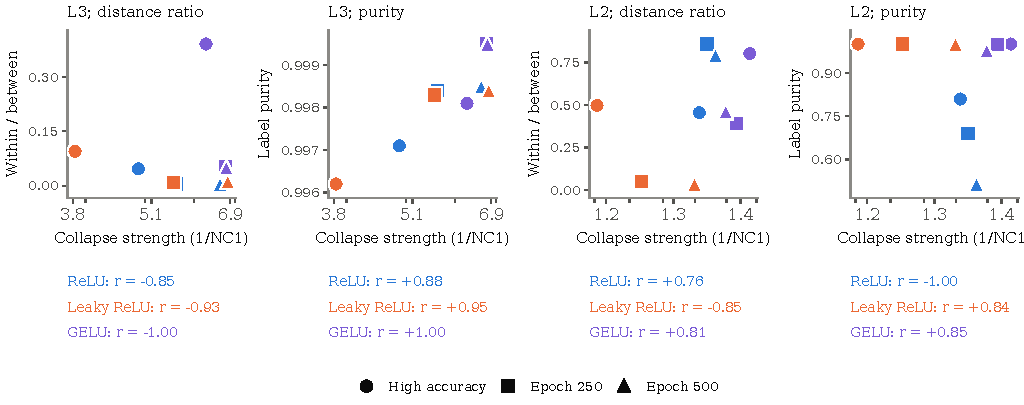
\includegraphics[width=6.147in]{nc_pairings.pdf}
\caption{Feature concentration versus downstream clustering in width-128 MNIST MLPs, seed 0. Larger $1/\mathrm{NC1}$ means stronger input-feature collapse; the horizontal scale is logarithmic. Points compare within-class/between-class downstream-map distance or diameter-cluster label purity at $\varepsilon=1$, at three matched checkpoints. Left pair: L3 maps and L2 features; right pair: L2 maps and L1 features. Colors identify activations and marker shapes identify stages. Each panel reports the within-activation Pearson correlation with $\log_{10}(1/\mathrm{NC1})$, using only these three points; a constant response has undefined correlation. These descriptive correlations do not establish a causal relationship.}\label{fig:nc-pairings}
\end{figure}
\FloatBarrier
